% !TeX root = ../0_Manuscript.tex

\section{Enhanced BBI platform in a fault attack context \ddcu}
\label{chap:2_goodPractices;sect:enhancedBBIGiraudAttack}
Now that we have seen with simple actual experiments the benefits of the proposed enhanced \bbi platform, let us linger on further experiments to verify more thoroughly the soundness of these enhancements.
To that end, I performed a differential fault attack on our IC target.
More specifically, a constraining fault attack requiring single bit faults on one or more bytes working on an AES cryptographic core, introduced by C. Giraud \cite{giraudDfa} in 2004.
In the first place, we are going to discuss in details the core of the attack.
Afterward, I will describe the IC target, its characteristics, and its operating conditions for the experiments.
Then, I will introduce experiments we developed to perform preliminary measurements to the attack, accelerating the search of points of interests on the IC.
Next, we will discuss the practical attack results.
Eventually, we will draw conclusions on the various observations.

    \subsection{Giraud's DFA detailed description \ddcu}
    When Giraud's paper \cite{giraudDfa} was published in 2004, no existing DFA was capable of attacking an AES algorithm.
    In this context, they proposed two types of DFA on AES, in order to cover various fault types one can induce on secured ICs.
    In this thesis, I focused on the first fault model, consisting in inducing single bit faults, therefore, this is the one we are going to discuss and describe in details in this section.

    % !TeX root = ../0_Manuscript.tex

\begin{figure}[H]
    \centering
    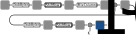
\includegraphics[width=0.8\textwidth, center]{2_goodPractices/figures/aesLastRounds.pdf}
    \caption{Two last rounds of an AES-128}
    \label{fig:aesLastRounds}
\end{figure}
    As we said before, the attack requires single bit faults on AES computation.
    More specifically, the fault has to appear at the beginning of the final AES round.
    Because we are using an AES-128, we will describe everything with this in mind.
    In addition to this, the various notations we will be using are the following:
    \begin{itemize}
        \setlength\itemsep{-0.1em}
        \item $P$ is the AES plaintext and $K$ the AES secret key
        \item $P^i$ stands for the intermediate cipher result after the $i^{th}$ AES round
        \item $P^i_j$ is the $j^{th}$ byte of $P^i$
        \item $K^i$ represents the $i^{th}$ AES round key
        \item As for $P$, $K^i_j$ is the $j^{th}$ byte of $K^i$
        \item $C$ is the correct ciphertext, $C_j$ is the $j^{th}$ byte of C
        \item Eventually, $CF$ stands for the faulty ciphertext, $CF_j$ is the $j^{th}$ byte of CF
    \end{itemize}
    Although the attack requires single bit faults on the final round, the attack is fairly simple and quick to perform with the right data at hand.
    I will not describe how AES operates, as it is well described in \cite{giraudDfa, aesRijndaelProp}.
    The final ciphertext is given thanks to the following equation:
    \begin{equation}
        \label{cipherGiraud1}
        C = ShiftRows(SubBytes(P^9)) \oplus K^{10}
    \end{equation}
    With $SubBytes(P^i_j)$ being the substitution table (S-box) result calculated on $M^i_j$ byte, and $ShiftRow(j)$ being the $j^{th}$ byte position of the temporary result of the $ShiftRows$ transform.
    Thanks to eqn. \ref{cipherGiraud1}, we can then deduce:
    \begin{equation}
        \label{cipherGiraud2}
        C_{ShiftRow(i)} = SubByte(P_i^9) \oplus K^{10}_{ShiftRows(i)}, \forall \in \llbracket0, 15\rrbracket
    \end{equation}
    If an attacker manages to induce a fault $e_j$ on a singe bit of the $j^{th}$ byte of the intermediate cipher $P^9$ before the AES final round, we have the following faulty ciphertext $CF$:
%    \begin{equation}
%        \label{faultyCipherGiraud1}
%        \begin{aligned}
%            & CF_{ShiftRow(j)} = SubByte(P_j^9 \oplus e_j) \oplus K^{10}_{ShiftRow(j)}\\
%            \implies & CF_{ShiftRow(i)} = SubByte(P^9_i) \oplus K^{10}_{ShiftRow(i)}, \forall \in \llbracket0, 15\rrbracket
%        \end{aligned}
%    \end{equation}
    \begin{equation}
        \label{faultyCipherGiraud1}
        CF_{ShiftRow(j)} = SubByte(P_j^9 \oplus e_j) \oplus K^{10}_{ShiftRow(j)}
    \end{equation}
    Which then gives us as before:
    \begin{equation}
        \label{faultyCipherGiraud2}
        CF_{ShiftRow(i)} = SubByte(P^9_i) \oplus K^{10}_{ShiftRow(i)}, \forall \in \llbracket0, 15\rrbracket
    \end{equation}
    If there is no fault on the $i^{th}$ byte of $P^9$, thanks to eqns. \ref{cipherGiraud2} and \ref{faultyCipherGiraud2}, we have the following relation:
    \begin{equation}
        \label{griaudNoByteFault_ith}
        C_{ShiftRow(i)} \oplus CF_{ShiftRow(i)} = 0
    \end{equation}
    If there is a fault on $P_j^9$, we have, thanks to eqns. \ref{cipherGiraud2} and \ref{faultyCipherGiraud1}:
    \begin{equation}
        \label{giraudFault}
        C_{ShiftRow(j)} \oplus CF_{ShiftRow(j)} = SubByte(P^9_j) \oplus SubByte(P^9_j \oplus e_j)
    \end{equation}
    Eventually, we have to first calculate ShiftRow(j), which gives us the location of the only non-zero byte of $C \oplus CF$, which in return gives us $j$.
    \textcolor{orange}{To finish.}

    \subsection{Integrated circuits target characteristics \ddcu}
    For the purpose of understanding clearly how we set up the previous attack, it is required to describe thoroughly the integrated circuit targeted.
    The model is an STM32F439VIT6 32-bits ARM Cortex-M4 microcontroller from STMicroelectronics, available in a LQFP100 package.
    The IC is manufactured using a 90 nm bulk technology.
    Its main characteristics are the following:
    \begin{itemize}
        \setlength\itemsep{-0.1em}
        \item A core clock up to 180 MHz
        \item Two 1 MB FLASH memory banks
        \item 256 kB of RAM
        \item Voltage supply allowed from 1.7 V to 3.6 V
        \item A True Random Number Generator (TRNG)
        \item A dedicated hardware cryptographic coprocessor, embedding AES (128, 192 and 256 bits), triple DES, and various HASH algorithms
    \end{itemize}
    For the purpose of every other experiment, the IC is clocked at 40 MHz thanks to an external 8 MHz crystal oscillator.

    \subsection{Preliminary attack experiments \ddcu}
        \subsubsection{Fault analysis mapping description \ddcnew}
        For the purpose of accelerating and simplifying the attack process, especially because creating single bit faults is a troublesome process, I designed experiments to be conducted on the IC target, allowing me to spot interesting IC areas to perform the attack on.
        Because the attack targets the AES coprocessor, all the experiments described here are performed specifically on the AES core area.
        % !TeX root = ../0_Manuscript.tex
%    trim={left lower right upper}
%\begin{figure}[H]
%    \centering
%%    \includegraphics[width=0.5\textwidth,
%%    trim={20cm 0cm 0cm 0cm},
%%    center]{2_goodPractices/figures/aesFastImpGnd.pdf}
%    \includegraphics[width=0.8\textwidth, center,
%    trim={14.9cm 0cm 0cm 0cm}, clip]{2_goodPractices/figures/aesFastImpGnd.pdf}
%    \caption{Fault susceptibility map analysis}
%    \label{fig:giraudFSM}
%\end{figure}

\begin{figure}[H]
    \centering
    \begin{subfigure}{0.49\textwidth}
        \includegraphics[width=\textwidth, center,
        trim={14.9cm 0cm 0cm 0cm}, clip]{2_goodPractices/figures/aesFastGndOnly.pdf}
        \caption{FAM: state-of-the-art}
        \label{fig:gndFSM}
    \end{subfigure}
    \begin{subfigure}{0.49\textwidth}
        \includegraphics[width=\textwidth, center,
        trim={14.9cm 0cm 0cm 0cm}, clip]{2_goodPractices/figures/aesFastImpGnd.pdf}
        \caption{FAM: enhanced}
        \label{fig:giraudFSM}
    \end{subfigure}
    \caption{Fault analysis mapping}
    \label{fig:fam}
\end{figure}

        These experiments are called "Fault Analysis Mapping" (FAM), and two results are shown in Fig.\ref{fig:fam}.
        An FAM consists in performing \bbi on the cryptographic core of the IC and identifying its behavior.
        We separated seven fault cases, described in Table \ref{table:faultType}.
        \begin{table}[H]
            \centering
            \begin{tabu}{|[2pt]l|[2pt]l|[2pt]}
                \tabucline[2pt]{-}
                Fault type           &  Description                                                 \\ \tabucline[2pt]{-}
                Correct              &  The AES outputs a correct result                            \\ \hline
                Monobit Monobyte     &  The fault is located on a single bit on a single byte       \\ \hline
                Multibit Monobyte    &  The faults are located multiple bits on a single byte       \\ \hline
                Monobit Multibyte    &  The faults are located multiple bytes and are single bit    \\ \hline
                Multibit Multibyte   &  The faults are located multiple bytes and multiple bits     \\ \hline
                Crash                &  The microcontroller did not respond correctly               \\ \hline
                Timeout              &  The microcontroller was unresponsive                        \\ \tabucline[2pt]{-}
            \end{tabu}
            %    \label{table:faultType}
            \caption{FAM faults description}
            \label{table:faultType}
        \end{table}
        Over the seven outcomes, only two of them can lead to potential exploitable fault according to Giraud's criterion: Monobit Monobyte and Monobit Multibyte.
        We performed these experiments on a state-of-the-art (default) platform and on our enhanced platform, with the exact same equipment on both platforms.

        \subsubsection{Fault analysis mapping comparison \ddcnew}
        FAM results are shown for the default platform in Fig. \ref{fig:gndFSM} and for the enhanced platform in Fig. \ref{fig:giraudFSM}.

        Concerning the state-of-the-art platform, where the FAM is shown in Fig. \ref{fig:gndFSM}, we can spot numerous locations where a microcontroller crash was observed, more specifically 70 \% of the tested locations.

    \textcolor{orange}{To finish.}
